\documentclass[conference]{IEEEtran}

\usepackage[noadjust]{cite}
%\usepackage[style=ieee,citestyle=ieee-comp]{biblatex}
\usepackage{amsmath}
\usepackage{amssymb}
\usepackage{graphicx}
\usepackage{tikz-cd}
\usepackage{booktabs}
\usepackage{multirow}
\usepackage{rotating}
\usepackage{array}
\usepackage{url}


\title{Explainable AI for Effective Malware Detection and Triage}

\author{\IEEEauthorblockN{Ananta Prasad Gaire, Aleksandar Shurbevski, Shozo Naito}

\IEEEauthorblockA{The Kyoto College of Graduate Studies for Informatics (KCGI)\\
Kyoto, Japan\\
Emails: st212678@m2.kcg.edu, a\_shurbevski@kcg.edu, s\_naito@kcg.edu}}

\begin{document}

\maketitle
\begin{abstract}
Security Operations Centers (SOCs) increasingly rely on machine learning to triage large volumes of potentially malicious artifacts, but operational use requires both strong discrimination and evidence that analysts can inspect. This report preserves the earlier PE-only WETICE-stage study and extends it with the current clean, multiformat EMBER2024 experiments requested during research supervision. The updated pipeline covers Win32, Win64, .NET, APK, ELF, and PDF files and combines the official 2,568-dimensional EMBER feature vector with a learned 64-dimensional structural embedding, producing a 2,632-dimensional fused representation for LightGBM classification. A provenance audit found exact duplicated halves in the local prepared shards; the local copy was therefore corrected to match the official EMBER2024 population of 2,626,000 training files and 606,000 temporally held-out test files. On the clean test set, the unified multimodal model achieves ROC-AUC 0.997668 and PR-AUC 0.997827. Following the supervisor's request for comparison with Joyce et al., we reconstructed predictions from the released EMBER2024 all-files LightGBM model on the identical 606,000-file test population and generated ROC curves for All, All PE, Win32, Win64, .NET, APK, ELF, and PDF partitions. The multimodal model improves ROC-AUC on all eight partitions, with the largest gain on APK (0.971962 to 0.984277), while low-FPR analysis reveals several operating-point-specific trade-offs that would be hidden by Accuracy or F1 alone. SHAP analysis shows that the structural embedding contributes 20.28\% of the aggregated mean absolute attribution despite representing only 64 of 2,632 input dimensions, and two structural dimensions are the highest-ranked individual features. Grad-CAM provides complementary localization evidence for the structural encoder, with the explicit limitation that it explains the CNN pathway rather than the final LightGBM decision. A completed true Win32 specialist experiment reaches ROC-AUC 0.998490 on 360,000 held-out Win32 files, closely matching the unified model's 0.998530. These findings extend the earlier PE-only work into a reproducible, multiformat, curve-based evaluation of explainable malware detection.
\end{abstract}

\section{Introduction}
\label{section:introduction}


%\subsection{Background and Motivation}

Modern organizations continuously receive, generate, and execute large volumes of digital artifacts through routine workflows such as software distribution, web browsing, and endpoint updates.
%In these workflows, 
Windows Portable Executable (PE) files are especially important from a defensive standpoint because PE is the native executable structure of Windows systems.
PE files remain a dominant malware delivery format~\cite{opentext2025} and can be distributed through common channels such as downloads, attachments, or bundled installers.
At Security Operations Center (SOC) scale, the challenge is not only detecting threats but doing so at a speed and volume that manual inspection cannot match.
To handle this scale, SOCs increasingly deploy~\cite{SDRS2025} machine learning (ML) systems to automate triage and prioritize suspicious files for analyst review.
Deep learning models are attractive in this setting because they can learn complex interactions in high-dimensional static features that rule-based filters and signature matching often miss~\cite{DSR2025ai}.
Yet, cybersecurity operations is a high-stakes environment: model outputs often influence decisions such as quarantining endpoints, blocking execution, or escalating incidents.
These actions require accountability, not merely high-confidence predictions.
If a model behaves as a black box and only provides a label (e.g., malware/benign), analysts face a trust gap: either they accept a decision they cannot justify, or they must re-investigate alerts from scratch, which reduces the operational value of automation.
The trust gap grows as threats evolve and adversaries manipulate surface cues.

%\subsection{Explainable AI and Its Role in Cybersecurity}

In this work, explainability is treated as evidence generation: model predictions are accompanied by feature-level and structural evidence that supports analyst verification, reporting, and triage.
%This is especially important in cybersecurity, where high-confidence predictions alone are often insufficient for operational decisions such as escalation, quarantine, or blocking.
For the implemented pipeline, SHAP is used to explain the final LightGBM~\cite{lightgbm} classifier, while Grad-CAM provides complementary structural evidence for the CNN image branch of the trained section model~\cite{LL2017,SCDVPB2017}.
Together, these methods help analysts inspect both \emph{which fused features mattered} and \emph{which structural regions were emphasized}.
Because explanation outputs are not automatically faithful, they must be interpreted carefully and supported by consistent preprocessing and evaluation design~\cite{JW2019}.

%\subsection{Research Aim and Scope}

This research aims to develop and evaluate an explainable, proposal-aligned pipeline for static malware detection from Windows PE artifacts.
The pipeline is designed to produce strong predictive performance and analyst-oriented evidence.
The work focuses on static detection using the EMBER2024 PE feature set~\cite{JMGPR2024} and a section-level structural representation derived from executables.
The scope does not include dynamic malware execution traces, malware family attribution, network intrusion detection, URL crawling, attachment sandboxing, sender reputation systems, or production SOC deployment engineering.

%\subsection{Design and Motivation}

%We study explainable static malware detection using EMBER2024 PE features~\cite{JMGPR2024}.
As a first modality we take the tabular PE representation already provided by the dataset.
The second modality is an image embedding derived from a compact section-structure representation processed by a CNN.
This design reflects the intuition that PE files contain both statistical feature evidence and structural evidence, and that combining both may improve detection while supporting richer analyst-facing explanations.
Accordingly, we compare a Tab-only baseline with a Tab+ImgEmb fusion model on the same held-out evaluation protocol.

% The comparative results are summarized in Table 1.
% 
% \begin{table}[htbp]
% \centering
% \small
% \setlength{\tabcolsep}{3pt}
% 
% \caption{Performance comparison on EMBER2024 malware detection}
% 
% \begin{tabular}{lccccc}
% 
%     \hline
% \textbf{Model} & \boldmath$\tau$ & \textbf{ACC} & \textbf{F1} & \textbf{ROC-AUC} \\
% \hline
% Tab-only LGBM (EMBERv3) & 0.50 & 0.9794 & 0.9792 & 0.9979 \\
% Tab + ImgEmb LGBM & 0.50 & 0.9795 & 0.9793 & 0.9979 \\
% Tuned Tab + ImgEmb LGBM & 0.35 & 0.9802 & 0.9801 & 0.9979 \\
% \hline
% \end{tabular}
% \label{tab:lgbm_small}

% \end{table}


We emphasize the tuned operating point because threshold selection is operationally important.
%, while still reporting the standard threshold for comparability. 
Explainability is integrated in a modality-aligned manner.
For the final Tab+ImgEmb LightGBM classifier, we use SHAP to generate explanation evidence over the fused feature vector, focusing on global feature rankings derived from the trained tree-based model~\cite{LL2017}.
For the image pathway, we use Grad-CAM~\cite{SCDVPB2017} on the CNN image branch of the trained section model to generate heatmaps that highlight structurally salient regions in the section-image representation.
%
%In the final code-backed pipeline, explanation reliability depends on keeping feature layouts, exported embeddings, and model artifacts aligned across inference and analysis.
%We therefore enforce artifact consistency so that reported probabilities and explanation outputs remain tied to the same trained pipeline.




\subsection*{Updated Research Scope}
The original WETICE-stage work concentrated on Windows PE artifacts and compared a tabular LightGBM baseline with a PE structural-image fusion model. That earlier experiment is retained in this report because it documents the development path of the research. The current study extends the same central hypothesis---that engineered static features and compact structural representations provide complementary evidence---to the complete EMBER2024 benchmark. The extension changes the evaluation question in three important ways: (i) all six official file types are included, (ii) final results use a corrected local copy whose counts exactly match the official dataset, and (iii) comparison with Joyce et al. is based on reconstructed ROC curves and low-FPR trade-offs rather than a single Accuracy or F1 value. The historical PE-only findings and the current clean multiformat findings are therefore reported as two phases rather than being mixed into one evaluation population.

\section{Related Work}
\label{section:literature-review}

Static malware detection sits at the front line~\cite{KBSSSK2025} of Security Operations Center (SOC) triage because it can be executed quickly, safely, and at scale, often before deeper investigation is feasible~\cite{GPH2024}.
For Windows endpoints, a large share of malicious delivery still arrives as Portable Executable (PE) files~\cite{opentext2025} distributed through downloads~\cite{recordedfuture2025malware}, attachments, and staged droppers.
Defenders must filter high-volume file streams with limited analyst time, and errors are costly.
This highlights the ML ``trust gap.''
On the one hand, deep models can achieve strong predictive metrics.
On the other, SOC decisions still require justification~\cite{NSDSP2025}: 
\begin{itemize}
 \item 
 why a file was quarantined, and 
 \item 
 what evidence supports that action.
\end{itemize}



Explainable AI (XAI) addresses this gap by producing interpretable signals (feature attributions and saliency maps) that connect model outputs to concrete input evidence.
In cybersecurity, this evidence supports analyst validation, accelerates investigation, and reduces reliance on opaque automation.
%For this reason, this research treats explainability as a first-class system output and evaluates XAI behavior as part of the overall malware detection pipeline~\cite{SCDVPB2017,LL2017}.

% \subsection{Static Malware Detection}
\subsection{Feature-engineered PE malware detection} % and the EMBER line of work}

A major practical tradition~\cite{HP20182018} in static malware detection is to extract specific, pre-defined properties from the Portable Executable (PE) file to create a fixed-length input vector.
In the literature, these inputs are variously referred to as ``handcrafted features''~\cite{MT2025,EDS2020}, ``engineered features''~\cite{HP20182018}, or ``tabular descriptors''~\cite{JMGPR2024}.
To maintain consistency and precision, we refer to them as \emph{engineered features}.
Engineered features typically include~\cite{KBSSSK2025} byte-level statistics (e.g., histograms), entropy-related measures that can correlate with packing/obfuscation, metadata derived from headers/sections, and import/export information that reflects program behavior at a coarse structural level.
The key strength of this approach is operational scalability: feature extraction and inference are fast~\cite{EDS2020}, and fixed-dimensional vectors support repeatable benchmarking~\cite{JMGPR2024}, thresholding, and controlled ablation studies~\cite{AQPWPWCR2022}.
The EMBER~\cite{HP20182018} dataset played a foundational role in making large-scale, reproducible PE-feature research possible by providing standardized feature extraction and evaluation conventions.
EMBER2024~\cite{JMGPR2024} extends this tradition by providing a large-scale, pre-computed dataset where each file is represented not as raw bytes, but as a vector of engineered values summarizing specific file characteristics.
These features explicitly include:
\begin{itemize}
\item 
Byte-level statistics:
Histograms and entropy calculations that capture the distribution of raw byte values.
\item 
Header information: 
Metadata extracted from the COFF and Optional headers (e.g., linker versions, timestamps, and machine types).
\item 
Section characteristics: 
Statistics regarding the size, entropy, and virtual memory layout of the executable's sections.
\item
Import and Export information: 
Hashed representations of imported libraries, imported functions, and exported symbols, which serve as proxies for the program's capabilities.
\end{itemize}
By relying on these pre-calculated engineered features, the EMBER2024 representation enables scalable training and systematic evaluation at the feature level~\cite{JMGPR2024,HP20182018}.

To support reproducible comparison, the EMBER2024 authors also provide official benchmark models and runnable training/evaluation scripts in a public repository~\cite{JMGPR2024,ember2024github}.
These baselines are primarily LightGBM classifiers trained on EMBER feature version 3 vectors, intended to serve as reference performance levels for future work.
For malicious/benign detection, the benchmark LightGBM classifier is reported to achieve ROC AUC = 0.9949 on the EMBER2024 test set~\cite{JMGPR2024},
while having a true positive rate of 94.48\% for a fixed 1\% false positive rate.
% For malware family classification, the benchmark LightGBM model reports accuracy = 67.97\%, with weighted-F1 = 0.6664 and macro-F1 = 0.4371, reflecting the long-tail difficulty across many smaller families~\cite{JMGPR2024}.
% These published baseline results provide a consistent reference point that later experimental results (including ours) should be compared against.

\subsection{Representation learning from raw bytes} % and the ``end-to-end'' alternative}

In parallel to engineered-feature pipelines, a competing research direction~\cite{RBSBCN2017,KBSSSK2025} argues that \emph{end-to-end} models operating directly on raw bytes can discover discriminative patterns without relying on explicit feature design.
MalConv~\cite{RBSBCN2017} is a widely cited example, demonstrating that convolutional architectures can ingest long byte sequences to classify executables.
This family of approaches has expanded the field's understanding~\cite{RCEJH2025,KBSSSK2025} of representation learning for malware, but it also highlights practical constraints that are important for SOC-facing systems:
\begin{itemize}
\item 
very long sequences increase compute and memory costs~\cite{EDS2020}, 
\item
truncation or padding choices can affect what the model learns~\cite{RBSBCN2017,AQPWPWCR2022}, and 
\item
mapping byte-level signals to analyst-friendly evidence can be challenging compared to structured PE features~\cite{NSDSP2025,AQPWPWCR2022}. 
\end{itemize}


\subsection{Malware-as-image and structural visual encodings}

Another influential branch of malware research transforms executables into image-like representations to enable CNN-based modeling~\cite{NKJMB2011,KBSSSK2025}.
Early work~\cite{NKJMB2011} showed that visualizing binaries as images can support classification by capturing texture-like patterns that emerge from byte structure.
More recent work~\cite{ZLSC2024} continues to explore image conversion techniques, sometimes combined with additional features -- showing that visual encodings can complement other representations when designed carefully.
The literature further establishes that image-based approaches offer distinct advantages for interpretability and fusion.
Research indicates that unlike purely tabular data, visual representations enable spatial explanation methods (e.g., Grad-CAM) that can highlight exactly which regions of a file structure influence the model's decision~\cite{SCDVPB2017,ZLSC2024}.
Furthermore, studies in multimodal learning suggest that combining these structural visual signals with engineered feature vectors creates a more robust detection system, as the two modalities capture complementary patterns statistical evidence from features and spatial evidence from structure ~\cite{NKJMB2011,ZLSC2024}.

\subsection{Multimodal and fusion modeling for static malware detection}

The literature increasingly suggests that no single static view fully captures malware behavior, especially under packing, obfuscation, and family diversity~\cite{ZLSC2024,KBSSSK2025}.
As a result, fusion architectures that combine complementary signals have become more common.
For example, research that jointly analyzes PE structure with entropy-related signals reflects the broader idea that combining structural and distributional properties can improve malware classification robustness~\cite{SZS25}.
More generally, fusion is attractive because it provides redundancy: when one modality is less informative for a sample (e.g., a heavily packed file), another modality may still retain useful evidence.
This trajectory in malware research supports the hypothesis that fusing structured PE vectors with compact structural visual representations can improve detection performance without abandoning interpretability~\cite{SZS25,SCDVPB2017}.
%By comparing tabular-only baselines against fusion architectures, recent studies aim to quantify exactly how much robustness is gained by integrating these complementary static views.

\subsection{Explainability for malware: feature attribution for the final classifier and localization for the CNN pathway}

As explainable AI becomes increasingly important in malware detection~\cite{KBSSSK2025,NSDSP2025}, explanation methods must be matched to the actual model architecture used at inference time.
Additive feature attribution methods, such as SHAP, are better aligned with a final classifier, because they quantify how each feature contributes to the model score~\cite{LL2017}.
For CNN-based components, Grad-CAM produces class-discriminative heatmaps that highlight which spatial regions in an image-like input most strongly influenced the network response~\cite{SCDVPB2017}.
In a fusion model the above distinction is important, because it separates explanation of the final decision from supporting structural evidence in the image pathway.

A critical point in XAI literature~\cite{DJRLXSWB2020,NSDSP2025} especially relevant to security is that explanation outputs must be reliable.
Sanity-check research shows that some saliency or explanation methods can fail in subtle ways (e.g., remaining similar even when model parameters or labels are randomized), motivating validation procedures rather than assuming explanation faithfulness by default~\cite{JJMIMB2018}.
%This supports the methodological choice to treat explanation generation and validation as part of system design rather than as a post-hoc analysis~\cite{SCDVPB2017,LL2017,JJMIMB2018}.

\subsection{Positioning and Our Contribution}

The malware literature shows a consistent trajectory: high-performing models increasingly rely on deep learning and richer representations, but operational adoption in cybersecurity still requires transparent evidence and explanation reliability.
EMBER-style PE feature benchmarks and multimodal fusion trends motivate our Tab-only baseline and Tab+ImgEmb fusion design, while SHAP and Grad-CAM provide explanation modalities aligned to the implemented pipeline~\cite{JMGPR2024,SZS25,SCDVPB2017,LL2017,HP20182018,NKJMB2011}.
This section motivates controlled and scalable representations, multimodal fusion, and measurable explanation outputs aligned with the implemented pipeline.

%%%% Think if the next paragraph should be here or in architecture
%%These trade-offs matter to our project design.
%%We stay within a controlled, fixed-dimensional representation (tabular PE vectors, plus a compact ``section image'' representation) to keep the pipeline scalable and explanation outputs interpretable.
%%In other words, rather than choosing between ``feature engineering'' and ``end-to-end bytes,'' our work treats representation choice as an operational design decision: maintain tractable inputs that can support stable training, controlled evaluation, and explanation artifacts that analysts can act on.
%%%%%%
%%
%%%% The following paragraph is about our model
%%In the implemented pipeline, the final malware decision is produced by a LightGBM fusion classifier rather than an end-to-end neural network.
%%Accordingly, additive feature attribution methods such as SHAP are better aligned with the final classifier because they quantify how each fused feature contributes to the model score~\cite{LL2017}.
%%For malware detection, this produces ranked feature evidence that can be summarized into analyst-readable global tables, with the current implementation centered on global SHAP summaries.
%%For CNN-based components, Grad-CAM produces class-discriminative heatmaps that highlight which spatial regions in an image-like input most strongly influenced the network response~\cite{SCDVPB2017}.
%%However, in the implemented pipeline, Grad-CAM is applied to the CNN image branch of the trained section model used to produce image-side evidence, while SHAP is used to explain the final LightGBM classifier.
%%This distinction is important because it separates explanation of the final decision from supporting structural evidence in the image pathway.
%%%%%%
%%
The main contributions of this study are:
%
\begin{itemize}
\item
An explainable multimodal static malware detection pipeline using EMBER2024 PE features, including a Tab-only LightGBM baseline and a Tab+ImgEmb LightGBM fusion model evaluated under both standard and tuned thresholds~\cite{JMGPR2024}.
\item 
A multimodal explanation strategy for malware analysis, combining SHAP for the final LightGBM fusion classifier and Grad-CAM for structural localization in the CNN-based section model~\cite{SCDVPB2017,LL2017}.
\item 
Reliability-focused implementation findings, including feature-schema and artifact consistency for stable malware scores and reproducible explanation outputs.
\item
A clean-data multiformat extension covering Win32, Win64, .NET, APK, ELF, and PDF files, with explicit provenance auditing and the official EMBER2024 temporal train/test population.
\item
A supervisor-requested benchmark reconstruction in which the released Joyce et al. all-files LightGBM model and our unified multimodal model are evaluated on the same 606,000 files using ROC curves and constrained low-FPR operating points.
\item
Updated XAI and specialist analyses, including SHAP over the final 2,632-dimensional fused classifier, Grad-CAM for the structural encoder, and a true Win32-only multimodal specialist trained and evaluated independently.
\end{itemize}

\section{Methodology}
\label{section:methodology}

\subsection{Research Progression and Evaluation Phases}
The methodology is organized into two phases. \textbf{Phase I} is the earlier PE-only WETICE-stage experiment retained from the original report. It used a tabular PE representation and a CNN-derived image embedding to establish the feasibility of multimodal fusion and XAI. \textbf{Phase II} is the current final experiment: the dataset is rebuilt to the official EMBER2024 counts, all six file types are included, the structural encoder is standardized to a 64-dimensional embedding, and the main comparison is performed against the released Joyce et al. benchmark on an identical temporally held-out test population. Phase II is the basis for the current conclusions; Phase I remains as historical evidence of the research progression.

\subsection{Phase I: Earlier PE-only Pipeline (Retained)}

This paper proposes and evaluates an Explainable AI (XAI) framework for static malware detection from Portable Executable (PE) artifacts.
The methodology reflects SOC requirements: high-volume detection under time constraints, with evidence for analyst validation and reporting.
The project treats explainability as a core output, not a post-hoc visualization, because security decisions require justification and traceability.
The methodology emphasizes scalability and multimodal evidence, using large-scale PE feature vectors and section-derived structural representations to study whether complementary static views improve robustness.
Evaluation is conducted under a consistent protocol and includes probability threshold analysis to reflect deployment-style trade-offs in security settings.

\subsection{Data Source and Dataset Representation}

Malware detection is implemented as a static detection problem using an EMBER2024-derived PE representation~\cite{JMGPR2024,ember2024github}.
Each executable is mapped to a fixed-dimensional feature vector with a binary benign/malicious label, enabling scalable batch inference and feature-level explanation.
% For large-scale processing, the dataset is handled in sharded form for training, validation, testing, and explanation generation.
% In the final code-backed pipeline, the LightGBM experiments use the full EMBERv3 tabular representation released with the scripts, and feature-schema consistency is enforced across preparation, inference, and explainability.

\subsection{Preprocessing and Feature Consistency}

% Preprocessing consistency is treated as a first-order requirement.
In the earlier PE-only code-backed pipeline, the tabular-only model used a fixed EMBERv3 feature layout, whereas the fusion model additionally used exported image embeddings generated by the section model.
The main implementation requirement is therefore strict feature-schema and artifact consistency across preparation, training, inference, threshold sweeping, and explanation generation.
In analyst-facing settings, mismatches in feature ordering, dimensionality, or embedding generation can distort both model scores and explanation outputs.

\subsection{Model Architectures}

To evaluate the benefit of multimodal evidence while retaining interpretability, the project implements two final code-backed models: a Tab-only LightGBM baseline and a Tab+ImgEmb LightGBM fusion model, as illustrated in Fig.~\ref{fig:architecture}.

The Tab-only baseline operates on the EMBERv3 tabular feature vector and predicts the malware probability directly from the fixed-length PE representation.
This baseline quantifies how much discriminative power is available from the engineered static PE features alone.

\begin{figure*}[h]
 \centering
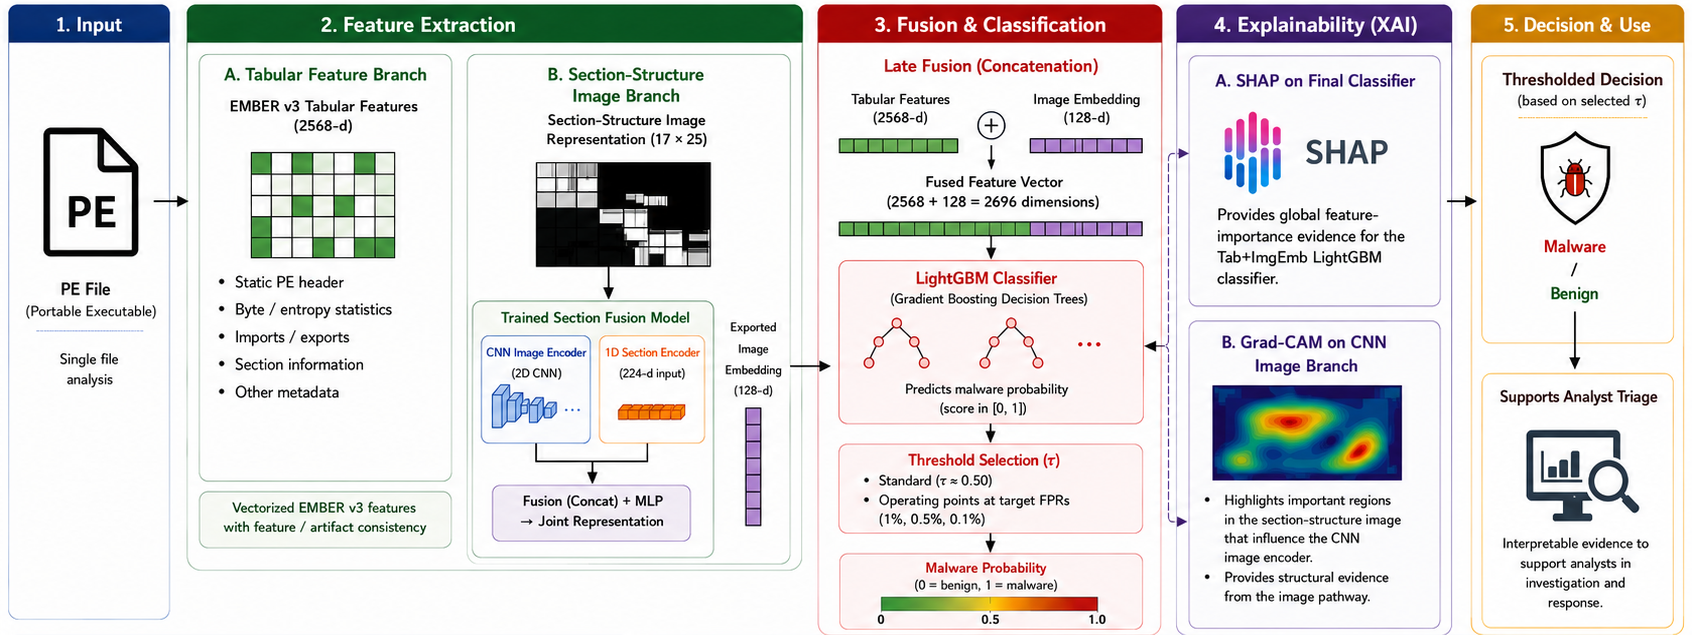
\includegraphics[width=0.99\textwidth]{figs/architecture_cropped.png}
\caption{Fusion model architecture.}
\label{fig:architecture}
\vspace{-3mm}

\end{figure*}


In Phase I, the Tab+ImgEmb fusion model combines two sources of evidence: the EMBERv3 tabular feature vector and an exported 128-dimensional image embedding derived from the CNN image branch of a trained section model operating on section-structure representations.
For each sample, the tabular feature vector is concatenated with the image embedding to form a fused feature vector, which is then passed to a LightGBM classifier to produce the final malware probability.
In the Phase-I pipeline, the tabular vector has dimensionality 2,568, the image embedding has dimensionality 128, and the resulting fusion vector has dimensionality 2,696.
This design preserves the complementary strengths of the two modalities: tabular PE features capture global structural and statistical signals, while the section model captures structural patterns that are summarized into the exported image embedding.


\subsection{Evaluation Protocol and Operational Thresholding}

Phase-I evaluation was performed on the earlier prepared PE-only test split of $960,000$ records. After the later provenance audit described below, these counts were recognized as belonging to the duplicated local preparation; the Phase-I metrics are retained for continuity, but final Phase-II claims use the corrected official-count population.
The models output malware probabilities, which are converted to binary decisions by comparing them to a threshold value~$\tau$.
Reporting both operating points reflects deployment-style trade-offs between missed malware and analyst workload.

\subsection{Explainability Methods}

We use two explanation methods aligned with the implemented malware pipeline: SHAP for the final LightGBM fusion classifier and Grad-CAM for the CNN image branch of the trained section model~\cite{LL2017,SCDVPB2017}.
Importantly for this research, the explainability pipeline is aligned with the feature fusion implementation:\\
- SHAP explains the final LightGBM decision, while\\
- Grad-CAM~\cite{LL2017,SCDVPB2017} provides complementary structural evidence from the CNN image branch of the trained section model.

For the final classifier, the input to LightGBM is a fusion vector formed by concatenating the EMBER tabular feature vector with the exported image embedding from the section model.
SHAP is applied directly to this trained tree-based model to measure how each fused feature dimension contributes to the malware score.
Global explanations are produced by computing mean absolute SHAP values over an explained sample subset, yielding a ranked summary of the most influential fused features.
The current implementation saves global SHAP summary artifacts for the final classifier.

Grad-CAM is not applied to the final LightGBM classifier itself.
Instead, it is applied to the CNN image pathway within the trained section model used to generate image-side evidence.
This produces structural heatmaps over the compact section-image representation, highlighting the regions that most strongly influence the CNN response.
In this way, SHAP explains the final fusion decision, while Grad-CAM provides complementary structural evidence from the image side of the system.



\subsection{Phase II: Clean EMBER2024 Population and Provenance Audit}
EMBER2024 contains 50,500 files per week across six file types. The official protocol uses the first 52 weeks for training and the final 12 weeks for testing, giving 2,626,000 training files and 606,000 test files~\cite{JMGPR2024,ember2024github}. During the full-dataset extension, our locally prepared raw shards initially contained exactly twice these counts. We therefore performed a shard-level provenance audit before retraining.

Across all 384 weekly file-type shards (312 train and 72 test), the first and second halves had identical SHA-256 sequences and identical binary labels. The feature-bearing fields used by the detection pipeline were also identical between the duplicated halves. The duplication was therefore treated as a local preparation issue, not a defect in the official EMBER2024 release. A clean local dataset was constructed by retaining the first half of each affected shard rather than deduplicating globally by SHA-256; this preserves any legitimate repeated hashes that may exist in the intended population. Table~\ref{tab:clean_counts} gives the resulting counts, which exactly match the official benchmark.

\begin{table}[t]
\centering
\caption{Clean EMBER2024 population used in Phase II.}
\label{tab:clean_counts}
\scriptsize
\renewcommand{\arraystretch}{1.08}
\begin{tabular}{lrr}
\toprule
\textbf{File type} & \textbf{Train} & \textbf{Test} \\
\midrule
Win32 & 1,560,000 & 360,000 \\
Win64 & 520,000 & 120,000 \\
.NET  & 260,000 & 60,000 \\
APK   & 208,000 & 48,000 \\
ELF   & 26,000 & 6,000 \\
PDF   & 52,000 & 12,000 \\
\midrule
\textbf{Total} & \textbf{2,626,000} & \textbf{606,000} \\
\bottomrule
\end{tabular}
\end{table}

The corrected dataset remains temporally ordered: training covers 24 September 2023 through 21 September 2024, while testing covers 22 September 2024 through 14 December 2024. This is important because the test files are later than all files used for training and validation, providing a more realistic temporal generalization setting than a random split.

\subsection{Phase II Tabular and Structural Representations}
The tabular branch uses the official EMBER feature version 3 vector with 2,568 dimensions. The feature layout contains general information, byte histogram, byte-entropy statistics, strings, PE header fields, section information, imports, exports, PE data directories, Rich-header features, Authenticode features, and PE parsing warnings~\cite{JMGPR2024,ember2024github}. Non-PE formats use the subset of EMBER features defined by the official extractor.

The second branch converts structural information into a fixed $17\times25$ representation together with a 256-dimensional structural vector. For Win32, Win64, and .NET, the rows summarize up to 16 PE sections plus an overlay row, while columns capture size, virtual-size, entropy, normalized ratios, section-name indicators, and section characteristics. For APK, ELF, and PDF, the representation uses byte-entropy and distributional summaries together with global metadata in the final row. Before encoder training, numeric structural values are converted to \texttt{float32}, non-finite values are normalized, signed $\log(1+|x|)$ scaling is applied where appropriate, and extreme values are clipped to stabilize convolutional training.

The structural encoder has two inputs: a CNN branch for the $17\times25$ structural representation and a one-dimensional branch for the 256-dimensional structural vector. Their hidden representations are fused and projected to a 64-dimensional embedding. The final classifier concatenates this embedding with the 2,568-dimensional EMBER vector:
\begin{equation}
\mathbf{x}_{\mathrm{fusion}} = [\mathbf{x}_{\mathrm{EMBER}};\mathbf{z}_{\mathrm{struct}}]
\in \mathbb{R}^{2632}.
\end{equation}
The structural encoder is trained with binary cross-entropy, Adam-style optimization, mixed precision, and a temporal validation split. The selected clean encoder achieved validation ROC-AUC 0.974021 at epoch 29.

\begin{figure*}[t]
\centering
\fbox{\parbox{0.95\textwidth}{\centering
\textbf{Phase-II multiformat fusion pipeline}\\[1mm]
Raw EMBER2024 JSONL $\rightarrow$ official 2,568-d tabular vector\\[1mm]
\hspace{14mm}$\searrow$ \hspace{36mm}$\swarrow$\\[-1mm]
\begin{tabular}{c@{\hspace{10mm}}c}
\textbf{Tabular branch} & \textbf{Structural branch}\\
EMBER v3 features & $17\times25$ structural representation + 256-d vector\\
$\mathbf{x}_{\mathrm{EMBER}}\in\mathbb{R}^{2568}$ & CNN + 1D encoder $\rightarrow\mathbf{z}_{\mathrm{struct}}\in\mathbb{R}^{64}$
\end{tabular}\\[1mm]
$\mathbf{x}_{\mathrm{EMBER}} \oplus \mathbf{z}_{\mathrm{struct}} \rightarrow$ 2,632-d fusion vector $\rightarrow$ LightGBM $\rightarrow$ malware probability\\[1mm]
SHAP $\rightarrow$ final LightGBM evidence \qquad Grad-CAM $\rightarrow$ structural CNN localization
}}
\caption{Current Phase-II multiformat architecture. The final decision is produced by LightGBM over the concatenated tabular and structural embedding.}
\label{fig:phase2_architecture}
\end{figure*}

\subsection{Fusion Classifier and Validation Protocol}
The selected Phase-II LightGBM uses up to 15,000 boosting iterations, learning rate 0.03, 256 leaves, minimum 100 samples per leaf, full feature and bagging fractions, $\lambda_2=1$, 96 CPU threads, and seed 42. Validation uses the final five weeks of the 52-week training period, leaving 2,373,500 files for fitting and 252,500 for validation. The selected model reached validation ROC-AUC 0.998029 and PR-AUC 0.998173 at iteration 14,578. A lower-learning-rate 20,000-iteration development run produced slightly lower validation ROC-AUC, so the 15,000-iteration configuration was retained before final test evaluation.

\subsection{Supervisor-requested Joyce et al. Reconstruction}
The supervisor specifically requested comparison with the non-image multimodal baseline of Joyce et al., with emphasis on ROC trade-offs rather than single Accuracy or F1 values. We therefore used the official EMBER2024 code and released benchmark models to reconstruct the Joyce all-files LightGBM predictions on the same clean 606,000-file test population~\cite{JMGPR2024,ember2024github}. The labels and file-type codes used for both methods were verified to be identical. Complete ROC curves were then generated for eight partitions: All files, All PE files, Win32, Win64, .NET, APK, ELF, and PDF.

For low-FPR reporting, we do not select the ROC point merely nearest to the requested FPR. Instead, for a target $\alpha$ we report
\begin{equation}
\max_{\tau}\;\mathrm{TPR}(\tau) \quad \text{subject to}\quad \mathrm{FPR}(\tau)\leq\alpha,
\end{equation}
for $\alpha\in\{0.01,0.005,0.001\}$. This constrained definition is conservative and directly answers the operational question: how much malware can be detected without exceeding a specified false-positive budget?

\subsection{Phase II Explainability Protocol}
SHAP is computed for the final LightGBM model over a 6,000-sample explanation set, 1,000 samples per file type. The fused feature vector contains 2,568 tabular dimensions and 64 structural embedding dimensions. Global importance is summarized using mean absolute SHAP values. Grad-CAM is generated separately from the trained structural encoder for three illustrative examples per file type (18 examples total). This separation is deliberate: SHAP explains the final classifier, whereas Grad-CAM only localizes evidence used within the CNN pathway. Grad-CAM is therefore supporting structural evidence and is not claimed to be a direct explanation of the final LightGBM score.

\section{Implementation and Results}
\label{section:implementation-and-results}

\subsection{Phase I: PE-only WETICE-stage Results (Retained)}
We evaluated two malware detection models: a Tab-only LightGBM baseline and a Tab+ImgEmb LightGBM fusion model that augments the same tabular evidence with an image embedding exported from the CNN image branch of a trained section model.
The design goal is practical: scalable inference for large volumes of files with analyst-facing evidence rather than a single opaque score.

% \subsubsection{Decision Rule, Threshold Sweep, and Reported Metrics}

For each test sample the model outputs a malware probability, which we compare against a threshold value $\tau$ to decide if a file is malicious or not (benign).
% Given a decision threshold $\tau$, the predicted label is $\widehat{y}_i(\tau)=1$ if $p_i \geq \tau$ and 0 otherwise.
From the resulting confusion matrix counts, with respect to the decision question malicious or not, we compute Accuracy, Precision, Recall, and F1.
Because operational malware detection often requires balancing false negatives (missed malware) against false positives (benign files escalated), we report results at a range of thresholds, as well as the top F1 operating point identified by sweeping $\tau$ over multiple values.

% \subsubsection{Final Test Performance}

Table~\ref{tab:model_comparison} retains the earlier Phase-I performance on the prepared PE-only test split.
At $\tau=0.50$, the model reaches Accuracy = 0.9795, Precision = 0.9875, Recall = 0.9713, and F1 = 0.9793; at the best-F1 operating point ($\tau=0.353$), recall rises to 0.9774 and F1 to 0.9801.
The table also reports thresholds for false-positive-rate regimes of at most 1\,\%, 0.5\,\%, and 0.1\,\%, showing that stricter thresholds increase precision but reduce recall.

\begin{table}[t]
\centering
\caption{Malware detection results on the EMBER2024 All PE files set at selected operating points.}
\label{tab:model_comparison}
\scriptsize
% \setlength{\tabcolsep}{1.8pt}
\renewcommand{\arraystretch}{1.1}
\begin{tabular}{@{}llllccccc@{}}
\toprule
\multicolumn{3}{@{}l}{\textbf{Model}} & \textbf{Operating Point} & \boldmath$\tau$ & \textbf{Acc.}  & \textbf{Prec.} & \textbf{Recall} & \textbf{F1} \\
\midrule

\multicolumn{3}{l}{\multirow{3}{*}{\begin{sideways} Tab-only \end{sideways}}} \hspace{-6em}
 &   $\mathrm{FPR}\leq 1\%$                     & 0.591 & 0.9783 & 0.9898 & 0.9666 & 0.9781 \\
 & & &  $\mathrm{FPR}\leq 0.5\%$                & 0.813 & 0.9721 & 0.9948 & 0.9491 & 0.9714 \\
 & & & $\mathrm{FPR}\leq 0.1\%$                 & 0.979 & 0.9424 & 0.9989 & 0.8858 & 0.9389 \\
 & & & top-F1 \tiny{($\mathrm{FPR}\!\approx\!1.78\%$)}   & 0.325 & 0.9802 & 0.9821 & 0.9783 & 0.9802 \\
 \midrule
\multicolumn{3}{l}{\multirow{4}{*}{%
  \rotatebox[origin=c]{90}{\shortstack{Tab \vspace{-0.2em} \\ \vspace{-0.2em} +\\  \vspace{-0.5em} ImgEmb}}%
}}
 &  $\mathrm{FPR}\leq 1\%$                      & 0.593 & 0.9784 & 0.9898 & 0.9668 & 0.9782 \\
 & & & $\mathrm{FPR}\leq 0.5\%$                 & 0.825 & 0.9723 & 0.9948 & 0.9496 & 0.9717 \\
 & & & $\mathrm{FPR}\leq 0.1\%$                 & 0.981 & 0.9428 & 0.9990 & 0.8865 & 0.9394 \\
 & & & top-F1 \tiny{($\mathrm{FPR}\!\approx\!1.70\%$)}   & 0.353 & 0.9802 & 0.9829 & 0.9774 & 0.9801 \\
\bottomrule
\end{tabular}
\vspace{-3mm}
\end{table}

Figure~\ref{fig:roc_curve} shows the ROC curve of the final Tab+ImgEmb model on the All PE files subset of the EMBER2024 dataset.
The model achieves ROC-AUC = 0.99795, indicating strong class separability across operating thresholds.
This threshold-independent view complements the fixed-threshold metrics in Table~\ref{tab:model_comparison}.
The final Tab+ImgEmb model also achieved PR-AUC = 0.99805, showing that precision remains high across the recall range.

\begin{figure}[htbp]
    \centering
    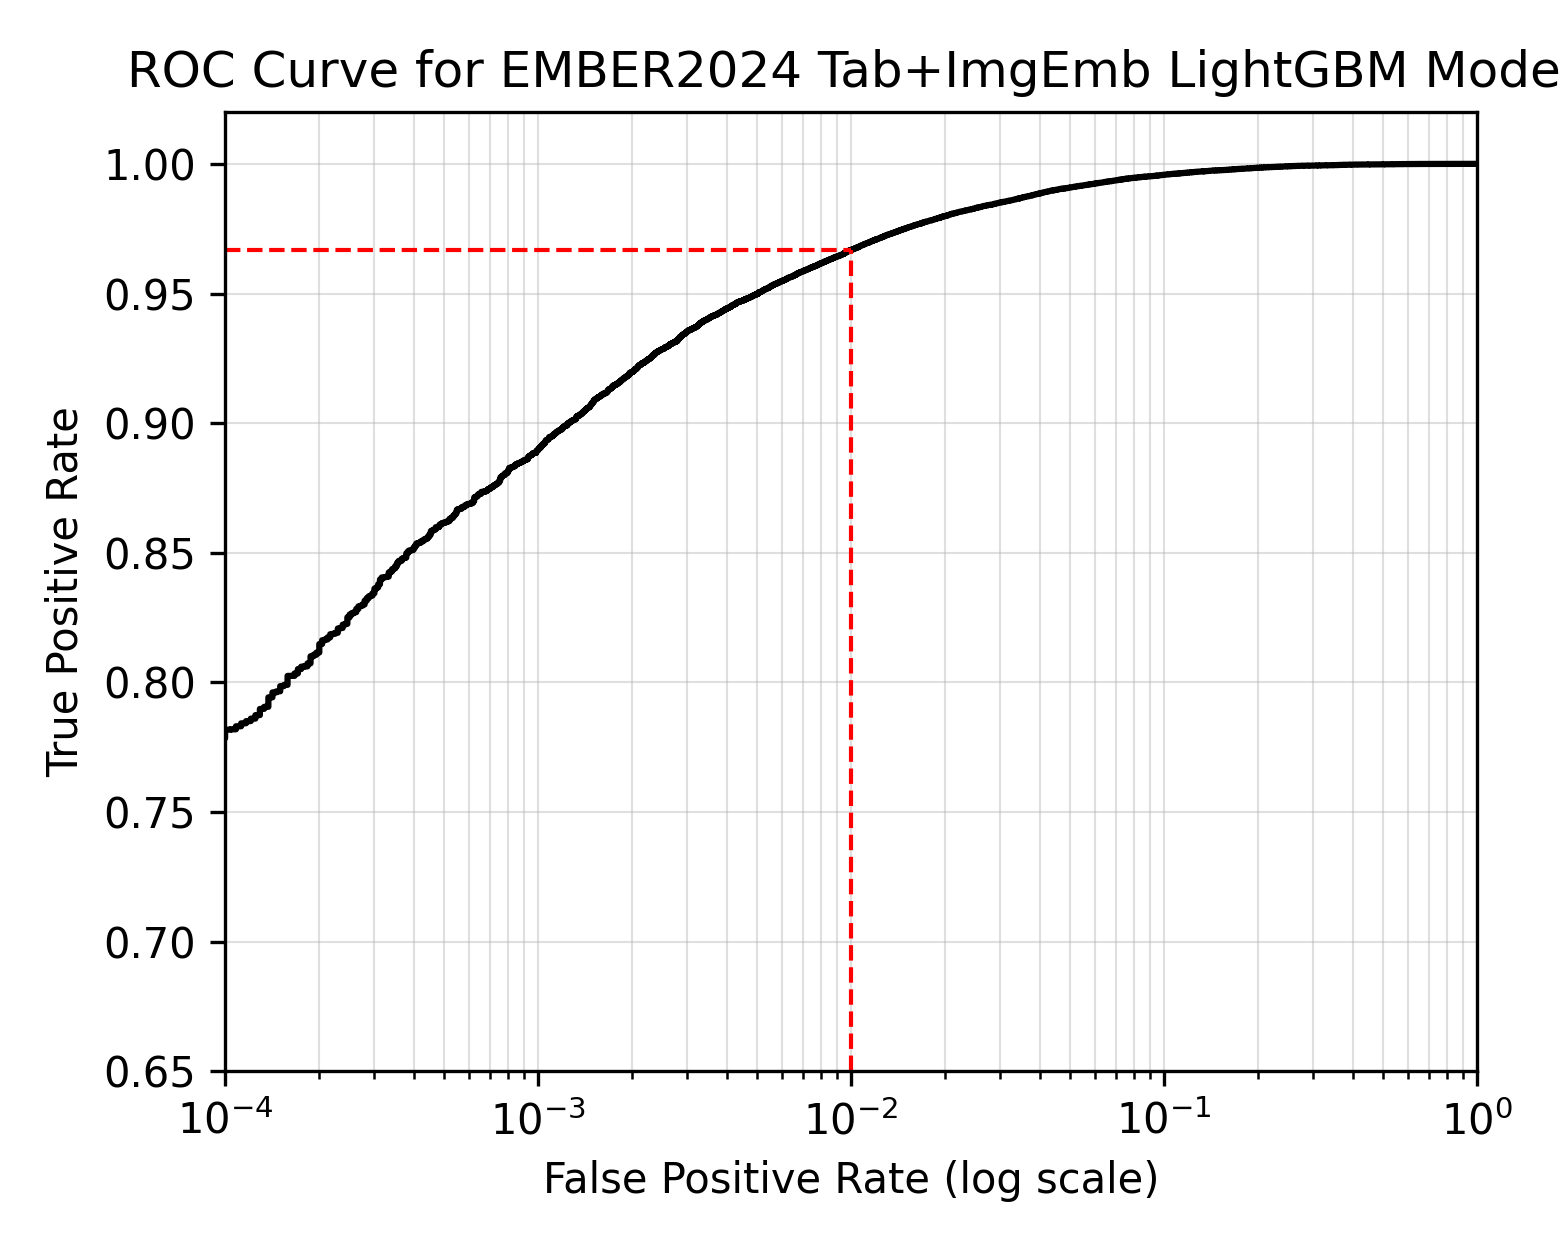
\includegraphics[width=0.39\textwidth]{curves/ROC_tab_plus_imgemb_full_test.png}
    \caption{ROC curve of the final Tab+ImgEmb model on the EMBER2024 all-PE test split (ROC-AUC = 0.99795).}
    \label{fig:roc_curve}
%\vspace{-3mm}
\end{figure}

The Phase-I result established that adding the structural image embedding could preserve strong discrimination while slightly improving operating-point behavior. Because the later provenance audit identified duplicated local records and Phase II expands the population to all six official file types, the current conclusions rely on the clean Phase-II evaluation below rather than on this historical threshold table.

% \subsubsection{Operational Interpretation}
% 
% Table~\ref{tab:operational_rates} summarizes operating-point behavior using rates rather than counts.
% As the threshold increases, FPR decreases, but TPR also decreases.
% At $\tau=0.353$, the model achieves TPR = 0.9774 at FPR = 0.0171, while at $\tau=0.500$ it reaches TPR = 0.9713 at FPR = 0.0123.
% At stricter thresholds such as $\tau=0.823$ and $\tau=0.979$, FPR falls to about 0.5\% and 0.1\%, respectively, but TPR also decreases.
% This makes threshold selection a practical choice between missed malware and analyst workload.

\begin{table}[t]
\centering
\caption{Operational rates for the final Tab+ImgEmb model on the EMBER2024 all-PE test set at selected thresholds.}
\label{tab:operational_rates}
\scriptsize
% \setlength{\tabcolsep}{6pt}
\renewcommand{\arraystretch}{1.1}
\begin{tabular}{@{}ccccc@{}}
\toprule
\boldmath$\tau$ & \textbf{TPR} & \textbf{FPR} & \textbf{TNR} & \textbf{FNR} \\
\midrule
0.353 & 0.9774 & 0.0171 & 0.9829 & 0.0226 \\
0.500 & 0.9713 & 0.0123 & 0.9877 & 0.0287 \\
0.593 & 0.9668 & 0.0100 & 0.9900 & 0.0332 \\
0.825 & 0.9496 & 0.0049 & 0.9950 & 0.0504 \\
0.981 & 0.8865 & 0.0009 & 0.9991 & 0.1135 \\
\bottomrule
\end{tabular}
\vspace{-5mm}
\end{table}

% At $\tau=0.353$, the model achieves TPR = 0.9774 at FPR = 0.0171, while at $\tau=0.500$ it reaches TPR = 0.9713 at FPR = 0.0123.
% At stricter thresholds such as $\tau=0.823$ and $\tau=0.979$, FPR decreases further, but TPR also declines.
% This makes threshold selection a practical deployment choice between missed malware and analyst workload.
% 
% \subsubsection{Explainability Report for Malware}


\begin{figure}[h!]    
  \centering
  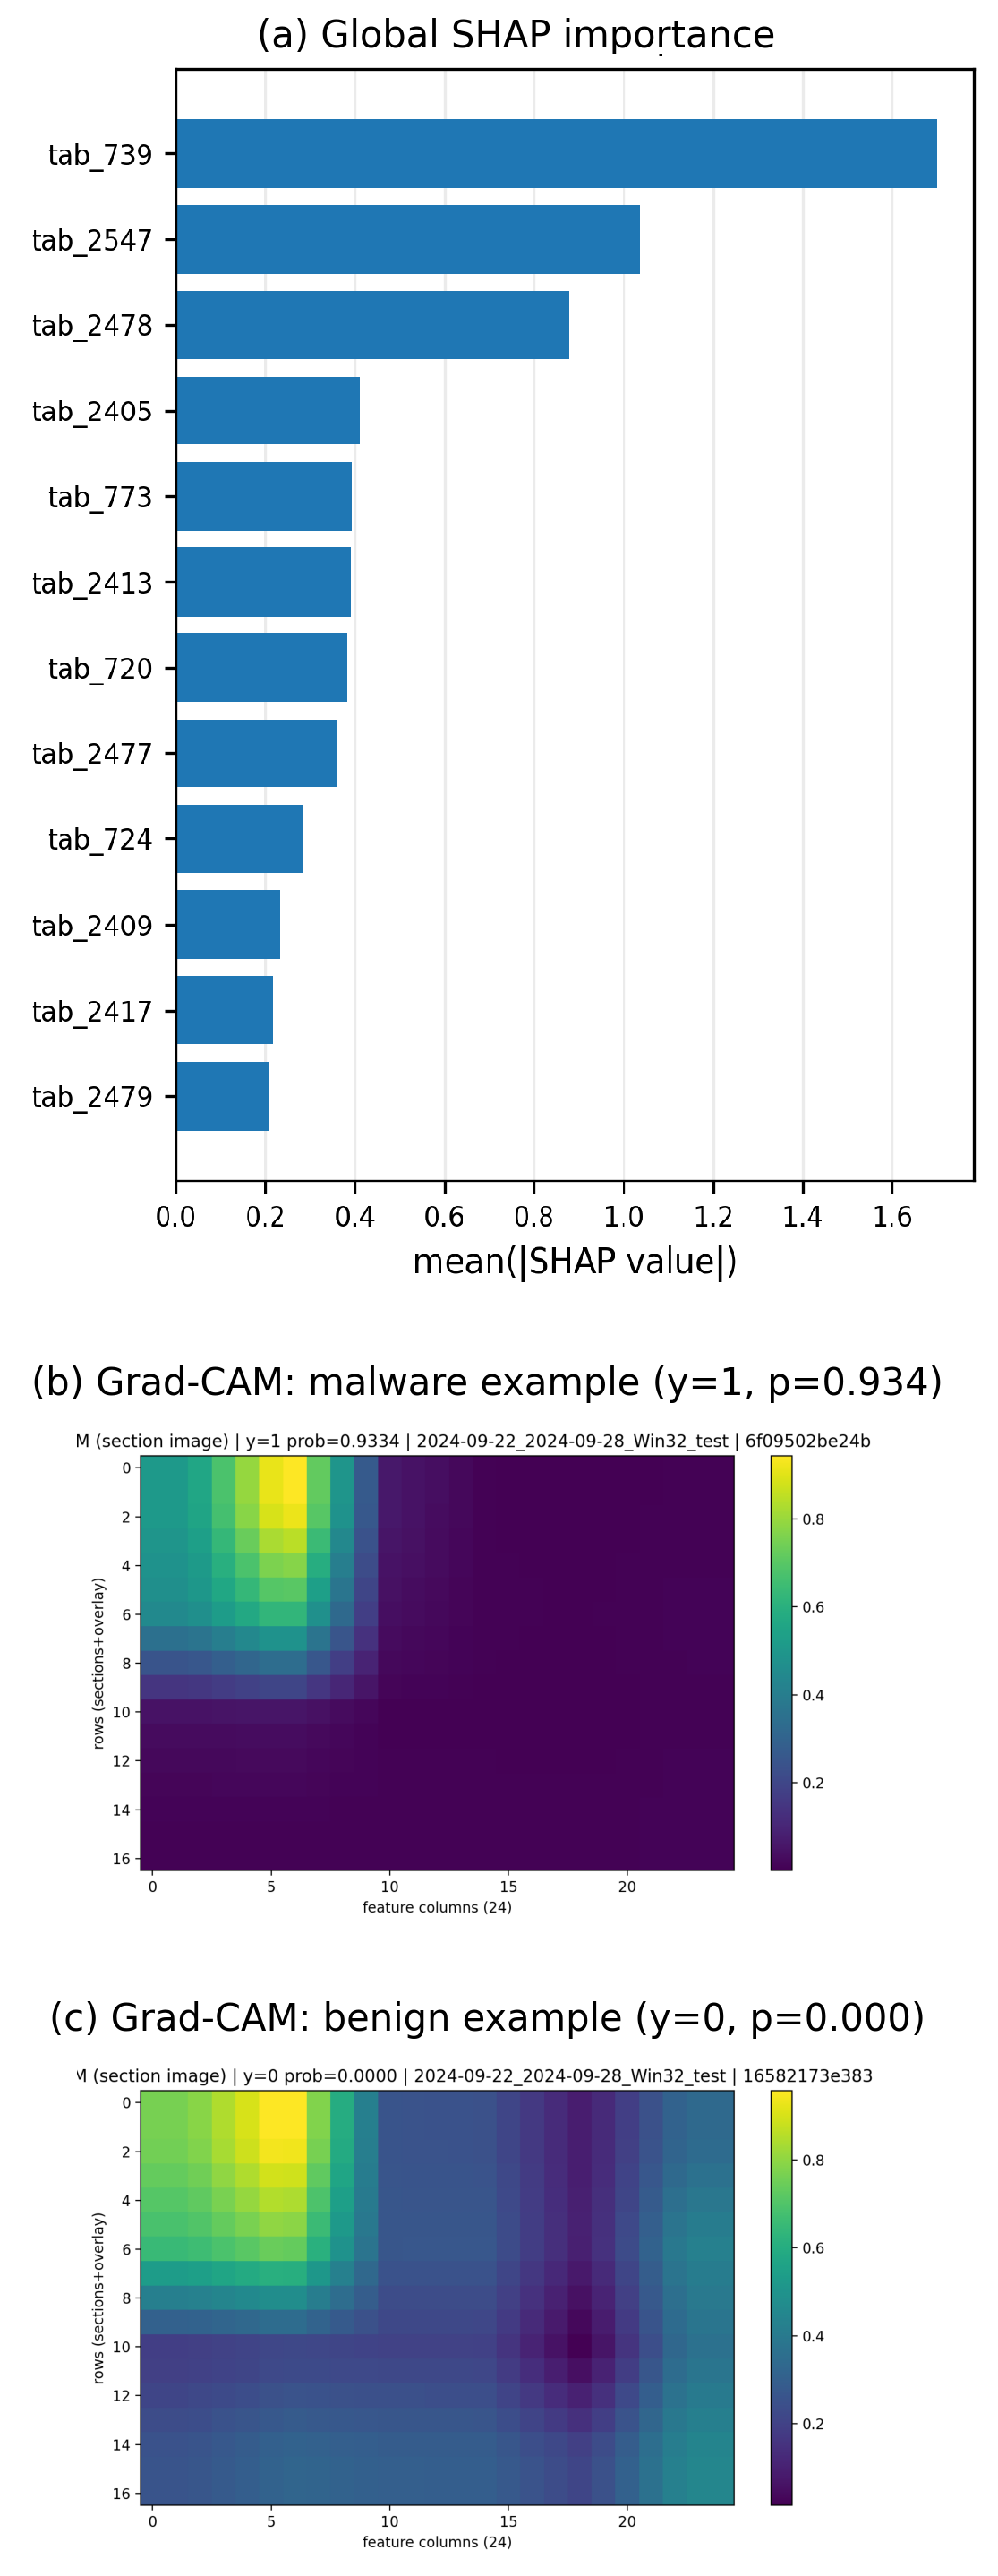
\includegraphics[width=0.35 \textwidth]{./figs/Figure_2_XAI_results_cropped.png}
  \caption{Explainability snapshot}
  \label{fig:xai}
  \vspace{-3mm}
\end{figure}

Explainability was implemented for both parts of the malware pipeline.
For the final Tab+ImgEmb LightGBM classifier, SHAP was used to generate global feature-importance evidence over the fused input vector.
For the image pathway, Grad-CAM was applied to the CNN image branch of the trained section model.
Thus, SHAP explains the final fusion decision, while Grad-CAM provides complementary structural evidence from the image pathway.
The output of our explainability stage is illustrated in Fig.~\ref{fig:xai}, where
in Fig.~\ref{fig:xai}\,(a) we see the most influential features of the tabular descriptors,
and in Figs.~\ref{fig:xai}\,(b) and~(c) show examples of the Grad-CAM visualization
for a malicious and a benign example, respectively.

In the implemented pipeline, the explainability results support two complementary views of a malware decision: which fused features contribute most strongly in the final classifier, and which structural regions are emphasized in the section-image pathway.

% \begin{table}[t]
% \centering
% \caption{Summary of explainability outputs in the implemented malware pipeline.}
% \label{tab:xai_summary}
% \scriptsize
% \setlength{\tabcolsep}{3pt}
% \renewcommand{\arraystretch}{1.0}
% \begin{tabular}{p{0.8cm}p{2.0cm}p{5.0cm}}
% \toprule
% \textbf{Method} & \textbf{Target} & \textbf{Observed role} \\
% \midrule
% SHAP & Final Tab+ImgEmb LGBM classifier & Provides global feature-importance evidence over the fused tabular and image-embedding input. \\
% Grad-CAM & CNN image branch of trained section model & Highlights structurally salient regions in the section-image representation used to produce image-side evidence. \\
% \bottomrule
% \end{tabular}
% \vspace{-5mm}
% \end{table}

These outputs improve transparency beyond a single score, while remaining supporting rather than causal evidence.

% \subsubsection{What the Malware Results Mean}
% 
% The malware results support three conclusions.
% First, the Tab+ImgEmb LightGBM fusion model consistently outperforms the tabular-only baseline, indicating that the image-embedding branch contributes complementary information rather than redundant noise.
% Second, the improvement is especially meaningful in recall: at $\tau=0.50$, the fusion model misses fewer malicious samples, which is important because false negatives are often the more costly error in security operations.
% Third, the explainability outputs make the model behavior more transparent: SHAP provides feature-level evidence for the final classifier, while Grad-CAM provides supporting structural evidence from the image pathway.


\subsection{Phase II: Unified Multiformat Test Results}
The final clean unified model was evaluated once on the complete 606,000-file temporal test set. Table~\ref{tab:phase2_metrics} reports threshold-independent ROC-AUC and PR-AUC together with the default $\tau=0.5$ operating point. The purpose of the threshold metrics is descriptive; the primary current comparison is the full ROC behavior and constrained low-FPR analysis requested by the supervisor.

\begin{table*}[t]
\centering
\caption{Phase-II clean unified multimodal results on the official-count EMBER2024 test set.}
\label{tab:phase2_metrics}
\scriptsize
\setlength{\tabcolsep}{4.0pt}
\renewcommand{\arraystretch}{1.08}
\begin{tabular}{lrrrrrrr}
\toprule
\textbf{Partition} & \textbf{N} & \textbf{ROC-AUC} & \textbf{PR-AUC} & \textbf{Accuracy} & \textbf{Precision} & \textbf{TPR} & \textbf{FPR} \\
\midrule
All files & 606,000 & 0.997668 & 0.997827 & 0.978140 & 0.985444 & 0.970617 & 0.014337 \\
All PE files & 540,000 & 0.998469 & 0.998579 & 0.982756 & 0.987610 & 0.977778 & 0.012267 \\
Win32 & 360,000 & 0.998530 & 0.998644 & 0.982528 & 0.989953 & 0.974950 & 0.009894 \\
Win64 & 120,000 & 0.998744 & 0.998845 & 0.985900 & 0.987541 & 0.984217 & 0.012417 \\
.NET & 60,000 & 0.997633 & 0.997716 & 0.977833 & 0.974010 & 0.981867 & 0.026200 \\
APK & 48,000 & 0.984277 & 0.985493 & 0.937458 & 0.965257 & 0.907583 & 0.032667 \\
ELF & 6,000 & 0.990000 & 0.990856 & 0.948000 & 0.937500 & 0.960000 & 0.064000 \\
PDF & 12,000 & 0.988305 & 0.990627 & 0.948250 & 0.989801 & 0.905833 & 0.009333 \\
\bottomrule
\end{tabular}
\end{table*}

The overall ROC-AUC of 0.997668 indicates strong separation across a heterogeneous population. Performance is highest on the PE-family partitions, but the unified model also remains strong on APK, ELF, and PDF. The lower default-threshold TPR for APK and PDF illustrates why a single global threshold is not sufficient for operational interpretation: a model can have a high ROC-AUC while a fixed threshold sits at a less favorable point on a particular file-type curve.

\subsection{Comparison with the Released Joyce et al. All-files Model}
Table~\ref{tab:joyce_auc} gives the direct unified-vs.-unified comparison. The reconstructed Joyce ROC-AUC values closely track the rounded values reported in the EMBER2024 work, although they are not numerically identical to the published table at every displayed decimal. We therefore distinguish \emph{reconstructed} scores from \emph{published rounded} values. All differences in Table~\ref{tab:joyce_auc} are computed from the reconstructed probabilities on the same clean vectors.

\begin{table}[t]
\centering
\caption{ROC-AUC comparison: released Joyce all-files LightGBM vs. our unified multimodal model.}
\label{tab:joyce_auc}
\scriptsize
\setlength{\tabcolsep}{3.5pt}
\begin{tabular}{lrrr}
\toprule
\textbf{Partition} & \textbf{Joyce} & \textbf{Ours} & \boldmath$\Delta$ \\
\midrule
All & 0.996819 & 0.997668 & +0.000849 \\
All PE & 0.998006 & 0.998469 & +0.000462 \\
Win32 & 0.998114 & 0.998530 & +0.000416 \\
Win64 & 0.998390 & 0.998744 & +0.000354 \\
.NET & 0.996702 & 0.997633 & +0.000931 \\
APK & 0.971962 & 0.984277 & +0.012315 \\
ELF & 0.987522 & 0.990000 & +0.002478 \\
PDF & 0.987761 & 0.988305 & +0.000545 \\
\bottomrule
\end{tabular}
\end{table}

The largest ROC-AUC gain occurs for APK (+0.012315), followed by ELF (+0.002478) and .NET (+0.000931). For Win32 and Win64, both models are already near the top of the ROC range, so the absolute AUC differences are necessarily small. These AUC results show that the structural representation adds discriminative information, but they do not imply that our model is superior at every possible false-positive budget. That question is addressed directly by the ROC curves and constrained operating points below.

\begin{figure*}[t]
\centering
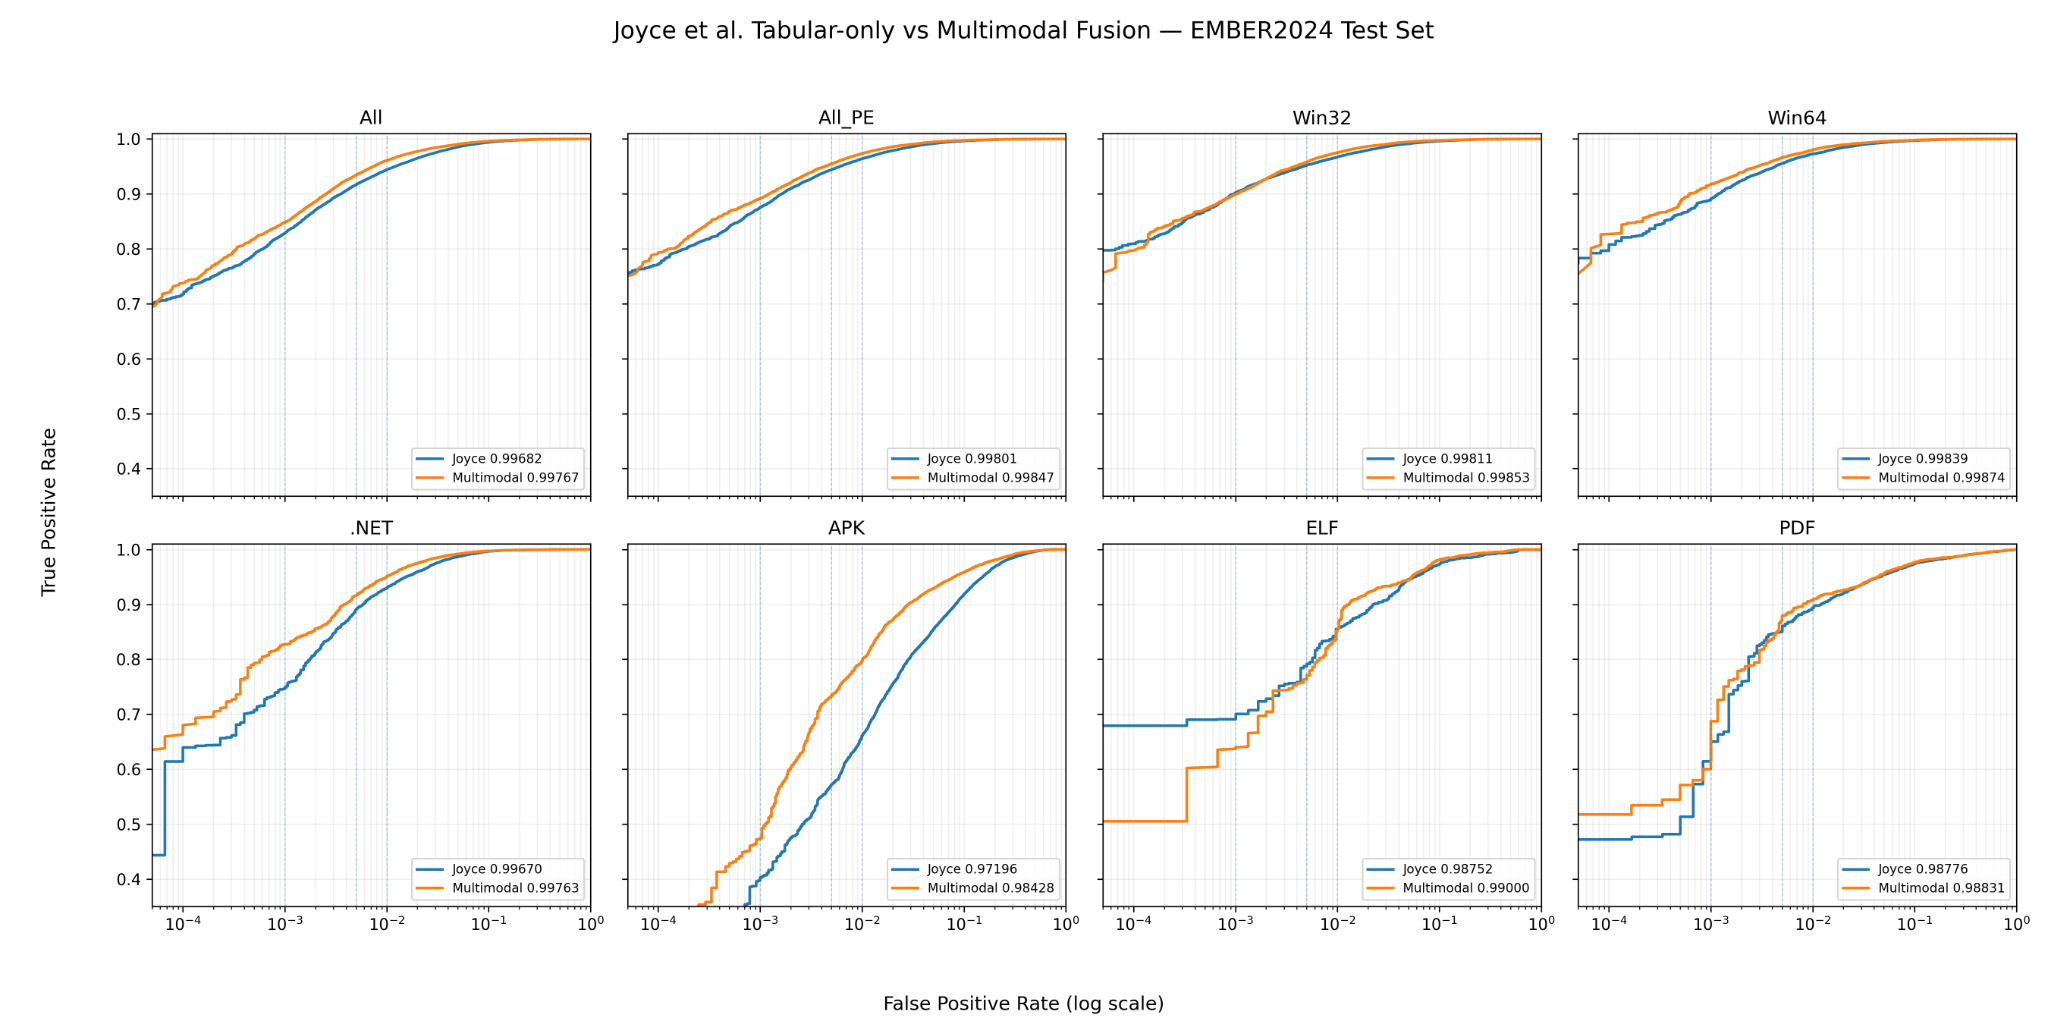
\includegraphics[width=0.98\textwidth]{figs/current/ROC_8_PARTITION_JOYCE_VS_MULTIMODAL.png}
\caption{Supervisor-requested ROC comparison of the released Joyce et al. all-files tabular LightGBM and the current unified multimodal model. Both methods are evaluated on the identical clean EMBER2024 test population. The horizontal axis is FPR on a log scale so that the low-FPR region is visible.}
\label{fig:joyce_roc8}
\end{figure*}

\subsection{Low-FPR Trade-offs}
Table~\ref{tab:lowfpr} reports the maximum TPR achievable without exceeding FPR limits of 1\%, 0.5\%, and 0.1\%. This directly implements the supervisor's preference for trade-off analysis rather than a single Accuracy/F1 operating point.

\begin{table*}[t]
\centering
\caption{Maximum TPR subject to a false-positive-rate constraint. Positive $\Delta$ means higher TPR for the multimodal model at the same FPR budget.}
\label{tab:lowfpr}
\scriptsize
\setlength{\tabcolsep}{3.4pt}
\renewcommand{\arraystretch}{1.08}
\begin{tabular}{lrrr|rrr|rrr}
\toprule
& \multicolumn{3}{c}{\textbf{FPR $\leq1\%$}} & \multicolumn{3}{c}{\textbf{FPR $\leq0.5\%$}} & \multicolumn{3}{c}{\textbf{FPR $\leq0.1\%$}} \\
\textbf{Partition} & \textbf{Joyce} & \textbf{Ours} & \boldmath$\Delta$ & \textbf{Joyce} & \textbf{Ours} & \boldmath$\Delta$ & \textbf{Joyce} & \textbf{Ours} & \boldmath$\Delta$ \\
\midrule
All & .9440 & .9608 & +.0168 & .9167 & .9341 & +.0174 & .8281 & .8485 & +.0204 \\
All PE & .9639 & .9734 & +.0096 & .9439 & .9548 & +.0109 & .8750 & .8916 & +.0166 \\
Win32 & .9671 & .9752 & +.0081 & .9522 & .9583 & +.0061 & .9021 & .8995 & -.0027 \\
Win64 & .9727 & .9802 & +.0074 & .9554 & .9664 & +.0109 & .8913 & .9174 & +.0261 \\
.NET & .9295 & .9509 & +.0214 & .8903 & .9167 & +.0265 & .7486 & .8273 & +.0787 \\
APK & .6609 & .7971 & +.1363 & .5715 & .7338 & +.1622 & .4027 & .4750 & +.0723 \\
ELF & .8560 & .8560 & .0000 & .7917 & .7707 & -.0210 & .7010 & .6397 & -.0613 \\
PDF & .8945 & .9083 & +.0138 & .8608 & .8792 & +.0183 & .6502 & .6872 & +.0370 \\
\bottomrule
\end{tabular}
\end{table*}

Three patterns are especially important. First, on the full 606,000-file population, multimodal fusion improves TPR by approximately 1.68, 1.74, and 2.04 percentage points at the three increasingly strict FPR limits. Second, APK shows the largest practical gain, especially at 0.5\% FPR where TPR increases from 0.5715 to 0.7338. Third, the gains are not universal: at the strictest 0.1\% FPR, Win32 is slightly lower, and ELF is lower at 0.5\% and 0.1\%. The ELF test partition contains only 6,000 files, so each false-positive increment has relatively large effect on the curve; nevertheless, the observed trade-off is reported rather than hidden.

\subsection{Updated Explainability Findings}
SHAP was recomputed for the clean Phase-II model using 6,000 samples. Summing mean absolute SHAP magnitudes by branch gives 34.223 for the tabular features and 8.706 for the structural embedding. Normalized by the total, these correspond to 79.72\% and 20.28\%, respectively. These percentages describe aggregate attribution magnitude, \emph{not} a decomposition of predictive accuracy.

The structural branch is highly compressed: it contributes only 64 of the 2,632 fused dimensions (2.43\% of the input dimensions) but 20.28\% of the aggregate absolute SHAP magnitude. Moreover, \texttt{struct\_emb\_1} and \texttt{struct\_emb\_38} are the two highest-ranked individual features, followed by \texttt{tab\_739}. Among the top 40 global SHAP features, 11 are structural embedding dimensions. This is evidence that the learned structural branch contributes information that the final LightGBM actively uses rather than being ignored after concatenation.

\begin{figure}[t]
\centering
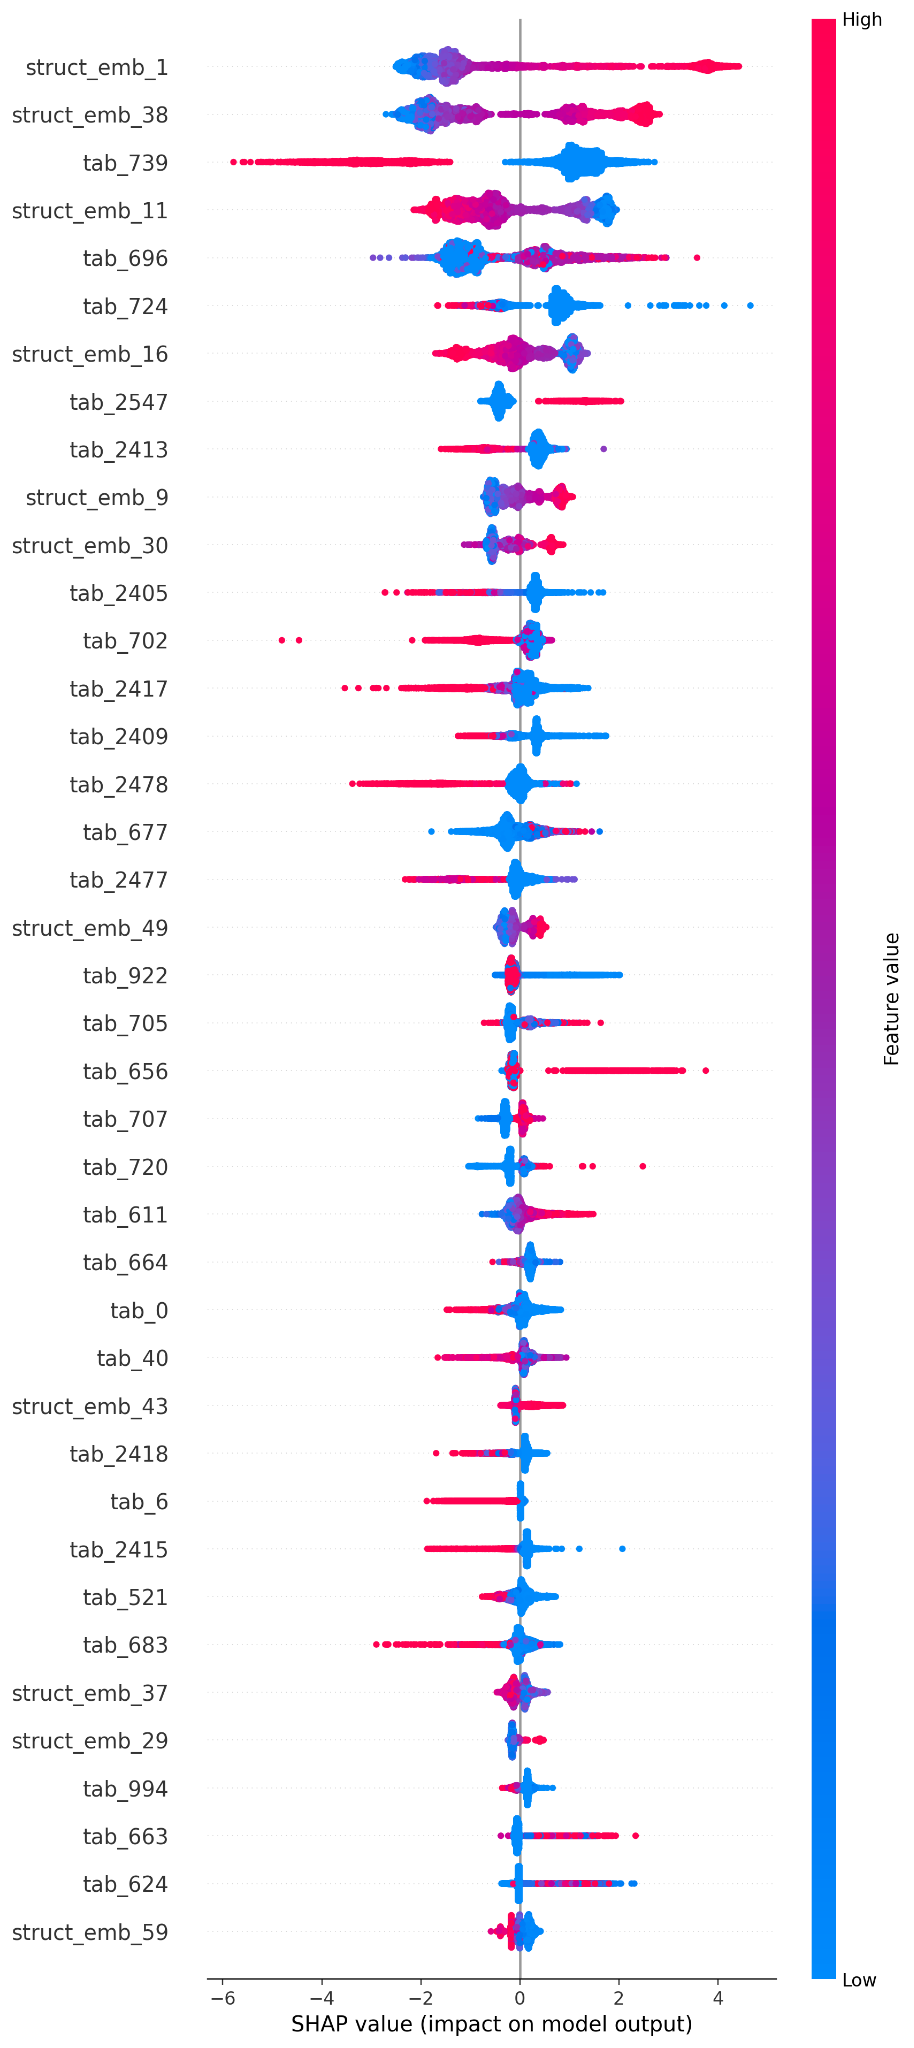
\includegraphics[width=0.46\textwidth]{figs/current/SHAP_multiformat_summary.png}
\caption{Global SHAP summary for the clean unified multiformat LightGBM. Structural embedding dimensions appear among the highest-impact features.}
\label{fig:phase2_shap}
\end{figure}

Grad-CAM was regenerated from the clean structural encoder for 18 illustrative test examples (three per file type). These maps visualize locations emphasized by the convolutional pathway in the $17\times25$ representation. Their interpretation is intentionally limited: because the final malware probability is produced by LightGBM after embedding export, Grad-CAM is evidence about the structural encoder, whereas SHAP is the explanation method aligned with the final classifier. This distinction is essential for faithful XAI reporting.

\subsection{True Win32 Specialist Experiment}
To begin a specialist-vs.-specialist study, a separate Win32 structural encoder and a separate Win32 fusion LightGBM were trained using only Win32 training data. This is a \emph{true specialist}: the representation learner itself is format-specific rather than reusing an encoder trained on mixed formats. The specialist encoder selected epoch 12 with validation ROC-AUC 0.984089. The fusion LightGBM used 1,410,000 Win32 files for fitting and 150,000 temporally later Win32 files for validation; its selected iteration was 5,328 with validation ROC-AUC 0.998638 and PR-AUC 0.998762.

On the untouched 360,000-file Win32 test partition, the specialist obtains ROC-AUC 0.998490 and PR-AUC 0.998622. At $\tau=0.5$, accuracy is 0.982925, precision 0.990581, TPR 0.975122, F1 0.982791, and FPR 0.009272. Table~\ref{tab:win32_specialist} places this result beside the unified models and the rounded Joyce Win32 specialist value reported in the benchmark study.

\begin{table}[t]
\centering
\caption{Win32 specialist status. Joyce specialist value is the published rounded ROC-AUC; reconstructed Joyce all-files and our models use the clean Win32 test partition.}
\label{tab:win32_specialist}
\scriptsize
\begin{tabular}{lr}
\toprule
\textbf{Model} & \textbf{Win32 ROC-AUC} \\
\midrule
Joyce all-files model (reconstructed) & 0.998114 \\
Joyce Win32 specialist (published) & 0.9984 \\
Our unified multimodal model & 0.998530 \\
Our Win32 multimodal specialist & 0.998490 \\
\bottomrule
\end{tabular}
\end{table}

The specialist is extremely close to the unified model but does not exceed it; the difference is approximately $4.1\times10^{-5}$ ROC-AUC. The result does not establish a causal explanation, but it is consistent with the possibility that cross-format training provides useful shared statistical regularization. More importantly, it shows that ``specialist'' should not be assumed to mean ``better.'' The remaining Win64, .NET, APK, ELF, and PDF true specialists are not reported as completed results because they have not yet passed the same train/validation/test process.

\subsection{Interpretation and Limitations of the Updated Findings}
The Phase-II results answer the supervisor's main methodological concern: the comparison is now curve-based, performed on identical test files, and emphasizes low-FPR behavior. The result is stronger than comparing rounded Accuracy or F1 values because it reveals where the models exchange ranking across operating regions. In particular, the multimodal model improves the overall curve and most constrained operating points, but the Win32 0.1\% FPR point and strict ELF points show that no single scalar summary captures the complete operational behavior.

Several limitations remain. The test set is temporally held out but still belongs to one benchmark collection period. The non-PE structural representation is a compact engineered visualization rather than a complete semantic parser for APK, ELF, or PDF internals. SHAP reports model attribution, not causal importance, and the Grad-CAM sample is illustrative rather than population-wide. Finally, the reconstructed Joyce results closely reproduce the benchmark but should not be described as bit-for-bit identical to every rounded published value; differences may arise from release state, preprocessing details, or rounding. For this reason, published and reconstructed benchmark numbers are labeled separately.

\subsection{Reproducibility and Artifact Traceability}
The updated pipeline records a manifest at each major stage: clean tabular vectors, structural modalities, encoder checkpoints, exported embeddings, LightGBM models, predictions, comparison curves, and XAI artifacts. Table~\ref{tab:artifact_stages} summarizes the main stages used for the current multiformat experiment. This structure was introduced specifically to prevent silent mismatches in feature ordering, data roots, or evaluation populations.

\begin{table}[t]
\centering
\caption{Main Phase-II reproducibility stages.}
\label{tab:artifact_stages}
\scriptsize
\begin{tabular}{lp{5.2cm}}
\toprule
\textbf{Stage} & \textbf{Purpose} \\
\midrule
Preflight/audit & Inventory file types, counts, schemas, and local duplication. \\
Vectorization & Build aligned 2,568-d EMBER vectors and labels. \\
Structural build & Create $17\times25$ representations and 256-d vectors. \\
Encoder & Train 64-d structural representation with temporal validation. \\
Embedding export & Freeze encoder and export train/test embeddings. \\
Fusion training & Train LightGBM on 2,632-d concatenated features. \\
Evaluation & Save labels, probabilities, type codes, metrics, and curves. \\
Joyce reconstruction & Run released benchmark model on the same clean test vectors. \\
XAI & Generate SHAP artifacts for final model and Grad-CAM for CNN pathway. \\
Specialists & Train format-specific encoder + LightGBM without test-set tuning. \\
\bottomrule
\end{tabular}
\end{table}

\section{Conclusion and Future Work}
\label{section:conclusion-and-futurework}

This report preserves the earlier PE-only WETICE-stage work and adds the completed clean multiformat extension requested during supervision. The central finding of Phase I remains useful: tabular EMBER features can be combined with a learned structural representation while retaining high malware-detection performance and producing complementary SHAP and Grad-CAM evidence. Phase II strengthens that result by rebuilding the experiment on the official-count EMBER2024 population and by evaluating the complete six-format test set.

The final unified model combines 2,568 official EMBER features with a 64-dimensional learned structural embedding and reaches ROC-AUC 0.997668 and PR-AUC 0.997827 on 606,000 temporally held-out files. Against the reconstructed released Joyce et al. all-files LightGBM, ROC-AUC is higher on all eight reported evaluation partitions. More importantly for the supervisor's request, the full ROC and constrained low-FPR analysis shows the actual trade-off: on the complete test population, TPR increases from 0.9440 to 0.9608 at FPR $\leq1\%$, from 0.9167 to 0.9341 at FPR $\leq0.5\%$, and from 0.8281 to 0.8485 at FPR $\leq0.1\%$. APK shows the largest low-FPR gains, whereas Win32 at the strictest 0.1\% FPR and ELF at the two strictest operating points show small reversals. Reporting these cases is important because they demonstrate why a single Accuracy or F1 value is insufficient for security evaluation.

The updated XAI results also support the multimodal design. Structural embedding dimensions account for 20.28\% of aggregate mean absolute SHAP attribution while comprising only 2.43\% of the fused dimensions, and two structural dimensions are the highest-ranked individual features. Grad-CAM complements this by localizing evidence in the structural encoder, but it is deliberately not presented as an explanation of the final LightGBM prediction. The completed Win32 true specialist reaches ROC-AUC 0.998490, nearly equal to the unified model's 0.998530 on the same Win32 test set, so the current evidence does not show a practical benefit from Win32-only specialization.

Future work should complete the remaining true specialists for Win64, .NET, APK, ELF, and PDF, reconstruct the corresponding released Joyce specialist ROC curves, and compare them under the same low-FPR constraints. Statistical uncertainty should be quantified with bootstrap confidence intervals or paired resampling on identical test files. Additional work should evaluate probability calibration, longer-term temporal drift, explanation stability over larger samples, and file-type-specific threshold policies. These extensions would move the system from a high-performing benchmark pipeline toward a more defensible analyst-facing malware triage system.

\bibliographystyle{IEEEtran}

\bibliography{references}

\end{document}
